\documentclass[12pt]{article}
\usepackage{styles/proposal}
\usepackage{styles/listofauthorships}
\usepackage{multicol}
% \usepackage[utf8]{inputenc}
\usepackage[style=ieee,citestyle=numeric-comp,sorting=anyt]{biblatex}
\graphicspath{{images/}}

\title{\scshape MQP Project Proposal}
\author{Samuel Goldman, Evan Goldstein, Christopher Myers, David Vollum}
% \date{September 2019}

% Glossary info goes in the preamble
\makeglossaries
% \todo{Fix numbering}
% Acronyms
% Follow the form: \newacronym{label}{ACRONYM}{expansion}
% Also: alphabetize!
\newacronym{api}{API}{application programming interface}
\newacronym{aws}{AWS}{Amazon Web Services}
\newacronym{caida}{CAIDA}{Center for Applied Internet Data Analysis}
\newacronym{cdf}{CDF}{cumulative distribution function}
\newacronym{cli}{CLI}{command-line interface}
\newacronym{cors}{CORS}{cross-origin resource sharing}
\newacronym{csv}{CSV}{comma separated value}
\newacronym{ddos}{DDoS}{distributed denial of service}
\newacronym{dns}{DNS}{domain name system}
\newacronym{dsl}{DSL}{digital subscriber line}
\newacronym{fcc}{FCC}{Federal Communications Commission}
\newacronym{gdp}{GDP}{gross domestic product}
\newacronym{gis}{GIS}{geographic information system}
\newacronym{gps}{GPS}{global positioning system}
\newacronym{html}{HTML}{Hypertext Markup Language}
\newacronym{http}{HTTP}{hypertext transfer protocol}
\newacronym{httpse}{HTTPS}{hypertext transfer protocol secure}
\newacronym{idw}{IDW}{inverse distance weighting}
\newacronym{iqr}{IQR}{inter-quartile range}
\newacronym{ip}{IP}{internet protocol}
\newacronym{ipaoc}{IPoAC}{internet protocol over avian carrier}
\newacronym{ipvs}{IPv6}{internet protocol version 6}
\newacronym{ipvf}{IPv4}{internet protocol version 4}
\newacronym{json}{JSON}{Javascript Object Notation}
\newacronym{jwt}{JWT}{\json Web Token}
\newacronym{mbps}{Mbps}{megabits per second}
\newacronym{mqp}{MQP}{major qualifying project}
\newacronym{ntp}{NTP}{Network Time Protocol}
\newacronym{ripe}{RIPE}{R\'eseaux IP Europ\'eens}
\newacronym{rtt}{RTT}{round trip time}
\newacronym{sdk}{SDK}{software development kit}
\newacronym{svg}{SVG}{scalable vector graphics}
\newacronym{tcp}{TCP}{transmission control protocol}
\newacronym{tld}{TLD}{top level domain}
\newacronym{tls}{TLS}{transport layer security}
\newacronym{ttl}{TTL}{time-to-live}
\newacronym{acUrl}{URL}{uniform resource locator}
\newacronym{us}{US}{United States}
\newacronym{usps}{USPS}{United States Postal Service}
\newacronym{voip}{VoIP}{voice over internet protocol}
\newacronym{wpi}{WPI}{Worcester Polytechnic Institute}

% Acronyms with definitions
% Follow the form: \newacronym{label}{ACRONYM}{expansion}{description}. Description appears in glossary only.
\newacronym{anova}{ANOVA}{analysis of variance}{Analysis of variance is a class of statistical models and methods for estimation, used to analyze the difference between the means of a sample. Although there are many types, they all fundamentally calculate the probability (a $p$ value) that two population means are equal}

\newacronym{cdn}{CDN}{content delivery network}{A content distribution network, sometimes called a Content Delivery Network, is a network of proxy servers that form a kind of cache used to enhance delivery of content to internet users. Although helpful for internet users, they complicate measurements of connectivity to websites \textit{actually} connecting to the site's servers}
 
\newacronym{cv}{CV}{coefficient of variation}{Coefficients of variation, or relative standard deviations, are defined as the ratio of the absolute value of the mean of a variable divided by its standard deviation: $\frac{\lvert\mu\rvert}{\sigma}$. CVs are dimensionless values that can be judged independent of the original source, making them useful for gauging the spread of any data set. The lower the CV, the lower the spread of the data and the better the quality}
 
\newacronym{ecc}{EC2}{Amazon Elastic Compute Cloud}{EC2 is a service from Amazon Web Services that provides virtual machines in the cloud for general-purpose or task optimized work. EC2 can be configured for different performance and pricing classes, as well as complex auto-scaling schemes or virtual private cloud setups}
 
\newacronym{etl}{ETL}{extract-transform-load}{Extract-transform-load is a generic procedure for extracting data, transforming it into a more useful format, and loading it into a large volume storage system, such as a database. The term closer describes an architecture rather than a specific algorithm}
 
\newacronym{icmp}{ICMP}{internet control message protocol}{Internet Control Message Protocol is a protocol designed for error reporting and other utility purposes across the internet, typically used most by routers and other intermediary devices}

\newacronym{isp}{ISP}{internet service provider}{An internet service provider is typically the "last mile" organization that provides a user with internet access --- otherwise known as a \textit{tier 3} ISP. They are distinct from tier 2 and tier 1 ISPs which are responsible for much of the internet backbone, although ISP corporations may operate on multiple tiers. Common ISPs in the US include AT\&T, Comcast, and Verizon}
 
\newacronym{kde}{KDE}{kernel density estimation}{Kernel density estimation is a technique for estimating the probability density function of a variable. Briefly, KDEs work by processing each measurement of a variable as if it was at the center of some given probability density function, e.g. a gaussian curve. These curves are then summed together to form one curve and normalized so the area underneath the curve is equal to 1. A KDE chart can be read in the same way as a histogram can, but the $y$ axis corresponds to a density instead of an absolute value. The advantage to using a KDE over a histogram is that KDEs are not vulnerable to binning effects (from choosing the wrong bin size) while histograms are}

% Glossary entries -- these should be more detailed.
% Follow the form: \newglossaryentry{LABEL}{name={NAME} description={YOUR TEXT HERE}}
% \newglossaryentry{favicon}{
%     name={favicon},
%     description={Favicons are small identifying images, typically logos or relevant UI elements, that most websites provide for browsers to place on tabs and bookmarks. Favicons are stored as .ico files (icons) and are either 16x16, 32x32, or 48x48. This small size makes them ideal for testing connection \rtt from a browser}
% }

% \newglossaryentry{backbone}{
%     name={internet backbone},
%     description={Internet backbone infrastructure consists of high speed principal data routes and the connected major computer networks and core routers. For any trip of serious distance (likely most connections, unless you happen to have a data center in your backyard), packets will inevitably pass through some element of the internet backbone}
% }

% \newglossaryentry{traceroute}{
%     name={traceroute},
%     description={A traceroute is a technique that shows the full path data takes to get from your computer to a remote server, and how long it takes to get to each server along the way. Traceroutes leverage \icmp and specifically-set \ttl values to inciteintermediate servers to respond with an \icmp packet indicating the data packet's \ttl has expired -- thereby giving away the server's presence along the route}
% }


% Bibliography goes in the preamble
\bibliography{references}


\begin{document}
    %%%%%%%%%%%%%%%%%%%%
    %%% FRONT MATTER %%%
    %%%%%%%%%%%%%%%%%%%%
    
    % Title page
    % TODO MAKE A FANCY TITLE PAGE
    \pagenumbering{gobble}
    \maketitle
    \newpage
    
    % Table of contents, list of figures
    \pagenumbering{roman}
    \tableofcontents\newpage
    % \listofauthorships
    \listoffigures
    \newpage
    
    % Switch to arabic page numbering, start headers, and one half spacing.
    \pagenumbering{arabic}
    \pagestyle{fancy}
    \onehalfspacing
    
    %%%%%%%%%%%%%%%%%%%%%%%%%%%
    %%% MAIN PAPER CONTENTS %%%
    %%%%%%%%%%%%%%%%%%%%%%%%%%%
    
    % TO ADD SIGNIFICANT CONTENT:
    % Add a .tex file under the text folder, put your stuff there, then \input it in the
    % spot where it should go. THIS MEANS YOU DON'T HAVE TO DEAL WITH ONE GIANT MANUSCRIPT!
    
    \section{Introduction}
There are many ways to define "Internet connectivity," and for each definition many ways to measure it. For example, you could focus on the user experience aspect of connectivity and place emphasis on measuring what a typical user would actually do, i.e. loading from domains, not \ip addresses and accepting that \cdns and load balancing exist. Additionally, \textit{most} users likely use the \textit{top} websites - user experience analysis would account for this.

On the other hand, a network-centric approach could focus on analyzing the backbones and topology of the internet. This data would be of little use to everyday users, but potentially valuable to network researchers and architects looking to improve connectivity across the country.

This document presents various options for both approaches including how data might be collected, processed, and analyzed.\newpage
    
    To measure internet connectivity, it's important to concretely define \textit{what} internet connectivity is. To that end we've put together a list of possible metrics for defining internet connectivity.

\section{RTT to all other locations}
\label{sec:definition_rtt_to_everywhere}

\RTT is a measure of how long a packet's round trip between source and destination is. It has a major effect on the apparent latency of a connection or the quality of a streaming application such as video streaming, video calls, \voip calls, and multiplayer gaming. Lower \rtts indicate a better connection and a more responsive internet experience.

By measuring a location's average \rtt to any other location, we can roughly determine that connection's average quality. For example, we might find that a particular source has an average \rtt of 50 ms while another has an average 150 ms, so we would say the second has a worse connection than the first.

\paragraph{Normalized by distance}
Average \rtt per location may be informative, but without normalization by distance, it doesn't tell us much about the infrastructure in the region of the measurement. That quality is a better indicator of internet connectivity than raw \rtts are because \rtts will be heavily affected by connections to far away geographic regions. For instance, a ping to a Chinese website will show an \rtt on the order of hundreds of milliseconds. Considering how far away China is and the amount of infrastructure between here and there, that's only to be expected. Averages at a location in the \us would be heavily swayed by those large values, meaning raw \rtt would misrepresent the data. The same applies to a user on the west coast trying to connect to a server on the east coast vs. the west coast. In reality the user's connectivity could be just fine, but by using a simple average or median of the two attempts, the data will be skewed somewhere in the middle.

To correct for this we can divide the average \rtt by the distance between source and destination to obtain a measurement of milliseconds per kilometer. Naturally this number will be very small, but it will be a good indicator of infrastructure in a region.

\section{RTT to regional locations}

It may be useful to group \rtt values by region, likely either by distance or national borders, based on the principle that an internet user will more likely connect to a server in the same country than to one in another country. In other words: Americans will likely visit American sites more than sites from other countries, so internet connectivity can be defined in terms of the sites a user would probably connect to. This measure of raw \rtt shares the same properties as raw \rtt from \cref{sec:definition_rtt_to_everywhere}, except with fewer high-\rtt destinations influencing averages.

\paragraph{Normalized by distance}
Just like raw global \rtts, regional \rtts can be normalized by distance. Average regional \rtt normalized by distance is a good measure of a region's connectivity within itself, which may or may not be a better indicator of typical internet connectivity for residents of that region.

\section{Aggregate RTT to /24 prefixes}

This metric would aggregate data for each /24 prefix into one data point, essentially merging 256 \ip addresses into a single node. This analysis would demonstrate average connectivity between /24 networks, similar in a way to analyzing connectivity between counties or zip codes. In doing so, it would characterize the overall connectivity of that network. Additionally, we should be able to link /24 networks to geographic areas and show which areas have the best and worst /24 prefixes.

\section{RTT to top websites}
Five websites (Google, Facebook, Youtube, Yahoo, and Amazon) dominate internet traffic in the \us with over 30\% of the traffic share \cite{Tachalova2017}. 67\% of \us internet users visit Google to search the internet and 68\% use Facebook for social media\todo[color=blue]{Citation needed}. These websites, along with the other top websites in the country, play a major role in internet connectivity and usability for a large portion of internet users in the United States. Therefore, measuring connectivity to these websites provides a window into the user experience of the internet for a geographic location.

Beyond the direct usage of top websites, major websites adopting \cdns contributes to internet consolidation. According to the Internet Society, 87.5\% of the top 1000 websites in 2018 used \cdns to speed up the delivery of their content. Of these 1000 sites, Amazon Cloudfront and Akamai provide \cdn services to 474 websites. The Internet Society states that four services (Dyn, Akamai, \AWS, and Cloudflare) serve an estimated 50\% of the top 1000 \texttt{.com}, \texttt{.net}, and \texttt{.org} domains \cite{TheInternetSociety2019}.

The reality of a more centralized internet is that, as the web grows ever more consolidated around these cloud services, the ability to speedily connect to any \ip address becomes less of an issue for everyday users. From this vantage point, a better internet connection is one that provides faster load times to the top content providers, regardless of their location. This metric is very similar to the \rtt measurements described in \ref{sec:definition_rtt_to_everywhere}, but is more focused on the end user's use case.

\paragraph{Normalized by distance}
While users might only care about the end result and how it impacts their ability to browse the web, normalizing the data by distance to the website data center could provide valuable information regarding regional infrastructure. A region showing high latency to top websites and a high ms/km rating might have room to improve, while a high latency region with low ms/km might not be able to improve. Network architects and companies looking to expand could use this data to prioritize locations and perhaps everyday users could use it to determine if their area has the potential to improve.

\section{Aggregate regional RTT to other regions}

This analysis would look at the average connectivity measurements (such as \rtt) in a political region to all other regions. These regions could be U.S. counties, zip codes, census blocks, or something else. Such aggregation doesn't necessarily follow the nature of network architecture, but this aggregation would highlight certain potential inequalities on political boundaries. Whatever these inequalities might be, focusing on these regions in this way would be useful to local authorities and constituents looking to improve internet access in their areas.

\section{Advertised speeds per region}
One of the things that can often dictate "internet connectivity" is the available "advertised" broadband connection speeds in a given region. It would provide an idea of both the infrastructure available area and what the \isp can successfully market. Advertised connection speed per region provide a strong metric into what average consumers can access across the US. Comparing the available advertised speeds between regions can show relative infrastructure differences.

\paragraph{Maximum}
The maximum available connection speed across an area gives an idea of what connections are possible in a given regional area. This metric can be used if money is not considered and all that is desired is the maximum possible connection speed without any throttling by the \isp.

\paragraph{Minimum}
The minimum connection speed available provides a strong summery of what would be considered to be the most accessible to every American.

\paragraph{Average}
The average advertised connection speed offered by Broadband subscribers in the \us provides a general metric for available speed across the \us. The metric would be the average of all of the connections offered for the given region. 

\section{Cost per megabit per second}
Internet infrastructure quality varies widely by location. Generally, urban areas have faster, more reliable and more stable infrastructure, and rural areas have slower, less reliable infrastructure. A good metric of the quality of the infrastructure is the cost per \mbps. The same speed connection will be (often significantly) more expensive in an area with a lower quality infrastructure (rural) than in an area with a higher quality infrastructure (urban). Comparing the cost per \mbps between different areas reveals the relative infrastructure quality between two different areas. This could also be considered a measure of user experience in the sense that a user must pay more for a better connection, resulting in a detriment to the overall internet usage experience.

% \subsection{Normalized by regional affluence}

\paragraph{Average}
The average cost per \mbps in an area can be used as a general metric for the internet connection quality in that area. An average should be taken across connections with "comparable" speeds and prices. For example, an average could include connections between 100 and 1000 \mbps and costs between \$50 and \$200/mo, and leave out outliers such as very expensive or inexpensive connections (relative to the area), or connections much faster or slower than most other connections (e.g. a 2 \mbps \dsl connection in an area where fiber is available). Multiple averages could be taken for a given area. For example, average cost of connections between 10 and 100 \mbps and betwen 100 and 1000. This would allow comparison of "fast" and "slow" connection speeds in two different areas.

% \subsection{Maximum}
% The maximum cost per \mbps in an area shows 

\section{RTT to backbone}

For all non-local traffic (likely the majority, since major data centers are relatively uncommon compared to residential locations) data will inevitably pass through the backbone, which will forward it on to its final destination. Backbone \rtt is then a measurement of how long it takes for a user to reach the nearest backbone entry point and vice versa, which should be a good indicator of internet connectivity and latency.

\paragraph{Normalized by distance}

Normalizing \rtt to backbone by distance is as useful as in other \rtt methods, since it gives a better picture of infrastructure quality between the user and the backbone. The effect of normalization will likely be diminished, however, since \rtt to backbone is technically a form of regional grouping.

\section{Data cap by region}

A data cap on broadband connections could reveal limited bandwidth in an area, and an attempt by the \isp to limit how much traffic consumers are generating. This is not a direct comparison, but possibly a correlation.

\section{IPv6 connectivity/availability}

Officially established as an internet standard in 2017, \ipvs expands \ipvf to 128 bits in order to address the exhaustion of 32 bit \ipvf addresses. However, deployment of network hardware that supports \ipvs has been slow. According to Google, as of September 2019, the \us has only reached 36.4\% adoption of the new protocol \cite{Google2019a}. While this is not an immediate problem, analyzing where \ipvs has not been implemented in the United States might show which regions are being prioritized. Overall, this definition of connectivity is a form of future internet connectivity.

\section{Risk of Disconnection/Stability of Connection}
Another way of looking at future connectivity involves determining how at risk a region is of becoming disconnected from the internet. A community or region may have sufficient connection now, but if that connection is reliant on a single point of failure (or any degree of failure lower than the rest of the population) in the network, its future connectivity is at risk. Another form of this, although less technical, would involve whether a government entity is capable and willing to sever or curtail internet availability.

\section{Content provider downtime by region}

Knowing how often content providers have downtime in different regions (likely at a state or larger scale) would show how reliable that region's connection to that content is. Differences between regions could be attributed to overall network reliability or any other of a number of issues. This again falls into the category of user experience and might be something that everyday users would be interested in learning about.
\newpage
    
    \section{Prior work}

% \subsection{FCC fixed broadband deployment map}
% The \FCC maintains a map of broadband internet deployment across the United States \cite{FederalCommunicationsCommission}. This map is drawn at a census block level and only considers residential broadband.
\newpage
    
    \section{Data Sources and Analysis Methods}
    \subsection{Favicon ping}[Samuel G.]
This method involves distributed users loading a web page that itself continually loads \glspl{favicon} from a set of predetermined, popular websites. favicons are small identifying images that most major websites provide for browsers to place on tabs. By loading these images with a random parameter to circumvent caching, the page can estimate the round trip time required to receive the favicon, analogous to a ping time. The site then reports this ping, along with the client \ip address, to a server.

Websites would likely be selected using a list of the most popular sites in the world and/or the United States, such as \href{www.alexa.com/topsites}{Alexa} or \href{www.similarweb.com/top-websites}{SimilarWeb}. Using such lists would focus this investigation on the websites that most impact usability of an internet connection for most people.

\paragraph{Potential issues}
Attempting to measure timing data from a browser will introduce jitter and uncertainty into the data, and estimated \rtts will not be representative of a true ping with \icmp packets. Additionally, the analysis might have to account for different browsers impacting load time, although we have not yet explored this.

\subsubsection{Multiple IP RTT}
When a user loads the data collection page, a script in the background will continually request favicons from a list of the top websites in the United States and measure the total time to get the image. This method only attempts to circumvent favicon caching (by including a randomized parameter) - it ignores the possibility of \cdns or any other methods of optimizing delivery speeds. We chose to include cache prevention because normal users don't repeatedly load favicons, however in order to collect enough data to eliminate jitter the favicon must be loaded multiple times for each user. By not accounting for \cdns, this method enables a limited form of normalization by distance: if a website uses a strong \cdn, it accounts for distance in load times, to a certain degree.

\paragraph{How the data is useful}
This data can show approximately how fast users can static resources from the top websites in the country. We can create maps showing connectivity for each targeted website, which would highlight differences for different websites. For example, users in San Francisco may have higher \rtts for wpi.edu than users in Boston. Additionally, averaging (perhaps with a weight based on popularity) the data for all websites together could show overall connectivity to the websites based on region. Conversely, for each website, this data can show which regions may need either stronger \cdn support or better network connectivity.

\subsubsection{Single IP RTT}
When a website uses a \cdn a client loading the web page on the east coast may end up loading Amazon.com's favicon from a different server than a user on the west coast. To circumvent this, the data collection site would load the favicons from a specific \ip address, bypassing \dns resolution.

\paragraph{How the data is useful}
Most people do not load websites from \ip addresses, so this method would not be representative of the experience for everyday users. However, this method has the potential to show the disparity in \cdns for different sites.

\subsubsection{Single IP RTT per distance}
When using the favicon ping method with a single target \ip, post analysis can estimate the approximate distance between the client and the server that sent the favicon. By dividing the average ping between that client and the server, we can normalize the data for distance.

\paragraph{How the data is useful}
While distance is a major factor in load times and overall user experience, normalizing for distance will highlight areas that have a better connection relative to their distance from content providers. However, this would not be representative of usability: users far from content data centers or \cdns would still suffer from slow load times even if they have a top tier connection. This analysis could show where efforts could be made to improve connections.

\subsubsection{Multiple IP RTT per rated connection speed}
Measured \rtt times to domain names (potentially multi-homed) could be normalized to expected connection speeds (see section below) using the size of the loaded favicon ((favicon size / (average rtt / 2) / expected connection speed). Using this data, locations could be assigned a "getting-what-you-paid-for" index. A higher value would indicate a better connection relative to the expected connection; a lower value would indicate connections worse than expected.

    \subsection{CAIDA, RIPE Atlas, \& Measurement Lab traceroutes}[Chris M.]

The \caida, \gls{ripe} Atlas, and Measurement Lab own nodes across the world that routinely run traceroutes to different locations. 

\caida maintains what they call the Archipelago network (or just Arc), a series \textapprox{}180 of Raspberry Pi's across the world that run measurements to different parts of the internet. We're interested in their prefix probing data set, which involves running complete traceroutes to at least one host in every /24 prefix. That is, every day, every Arc node runs a traceroute that picks up on one host in 130.215.1.x address, one in 130.215.2.x, and so on. This produces an \textit{enormous} amount of data, dating back to 2014 with over 6,000 compressed binary files. We have a series of python scripts that can extract this data and shove it into either hundreds of SQLite databases, or one big PostgreSQL database for easier analysis.

\gls{ripe} Atlas and Measurement Lab run on approximately the same principle, collecting tens of thousands of traceroutes per day.

To gain a better understanding of the data from \caida we conducted some basic statistic analyses to gauge the spread of the data. The charts below were created using about a sixth of the data available, with only source to final destination routes considered -- effectively just a ping.

\begin{figure}[H]
    \centering
    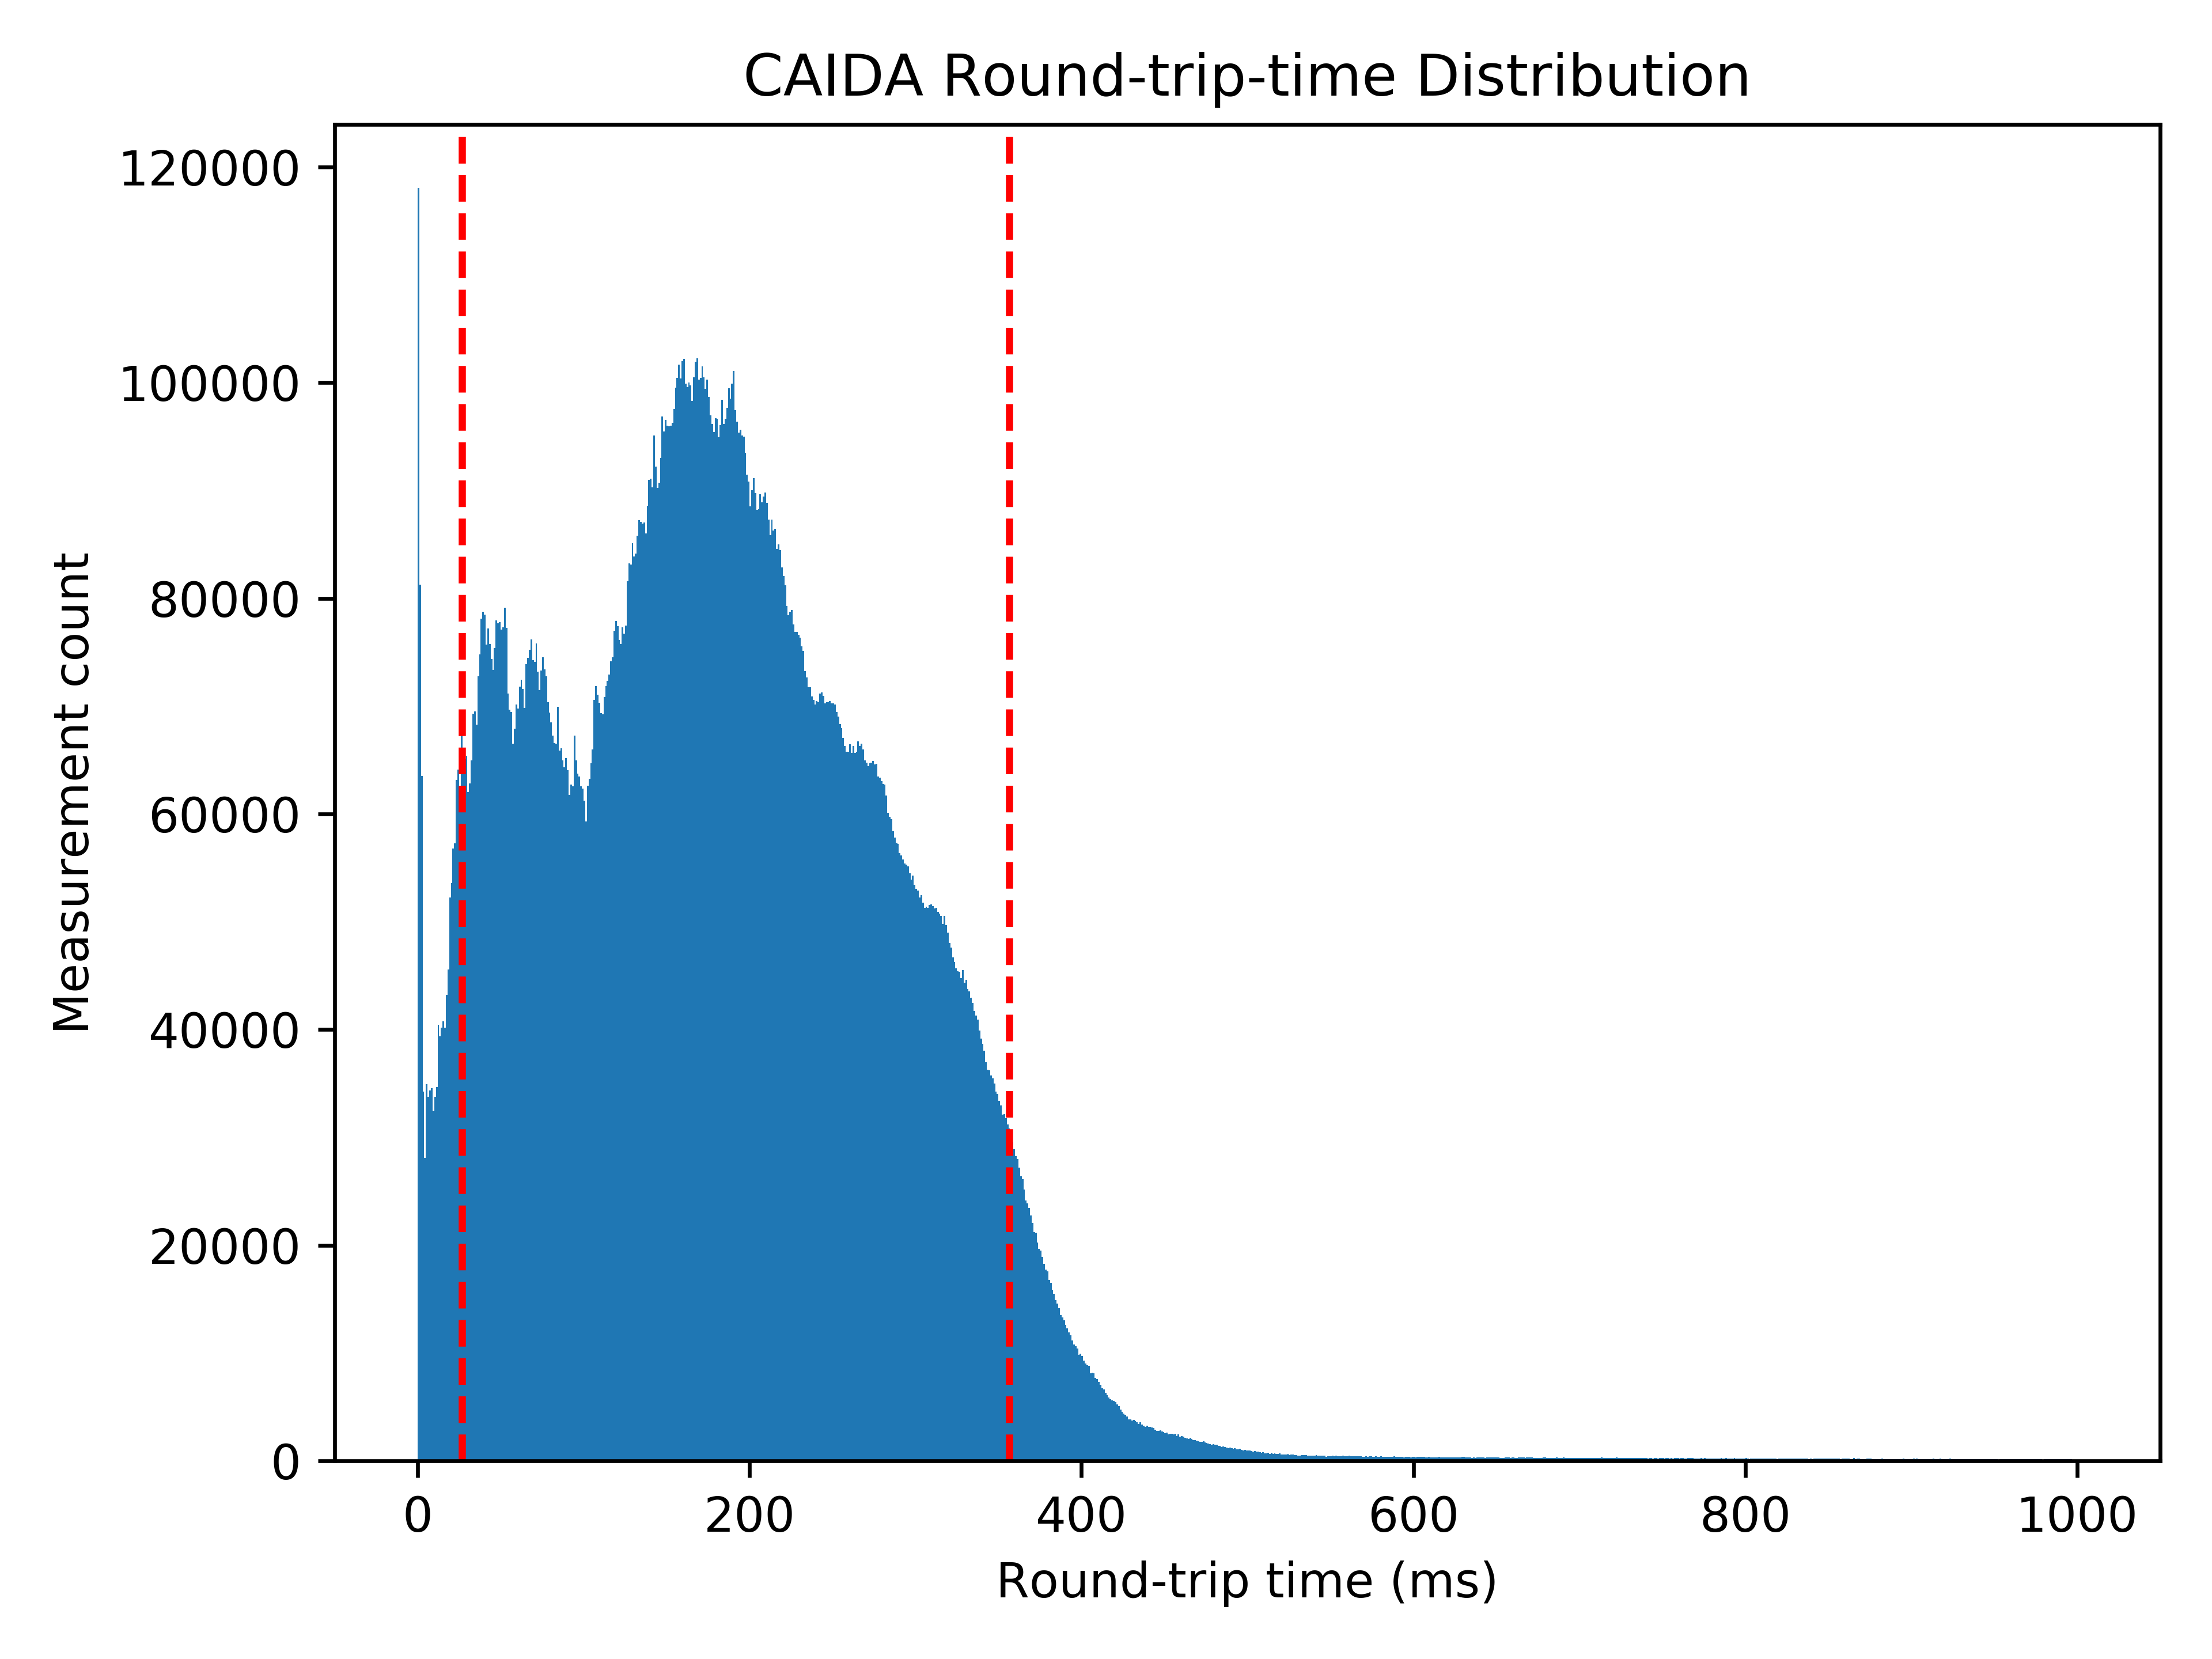
\includegraphics[width=\textwidth]{CAIDA_rtt_dist.png}
    \caption{Distribution of CAIDA RTTs with 5th and 95th percentiles shown}
    \label{fig:rtt_dist}
\end{figure}

Figure \ref{fig:rtt_dist} shows the distribution of \rtts recorded by CAIDA, with extreme values above 1000 ms omitted. The graph shows a reasonably sharp peak with a curious bimodal distribution. Fortunately, this easily explainable -- the two peaks likely represent sources from different landmasses. For instance, the larger peak on the right might correspond to hosts in Europe and Asia, while the smaller peak on the left might correspond to North and South America.

\begin{figure}[H]
    \centering
    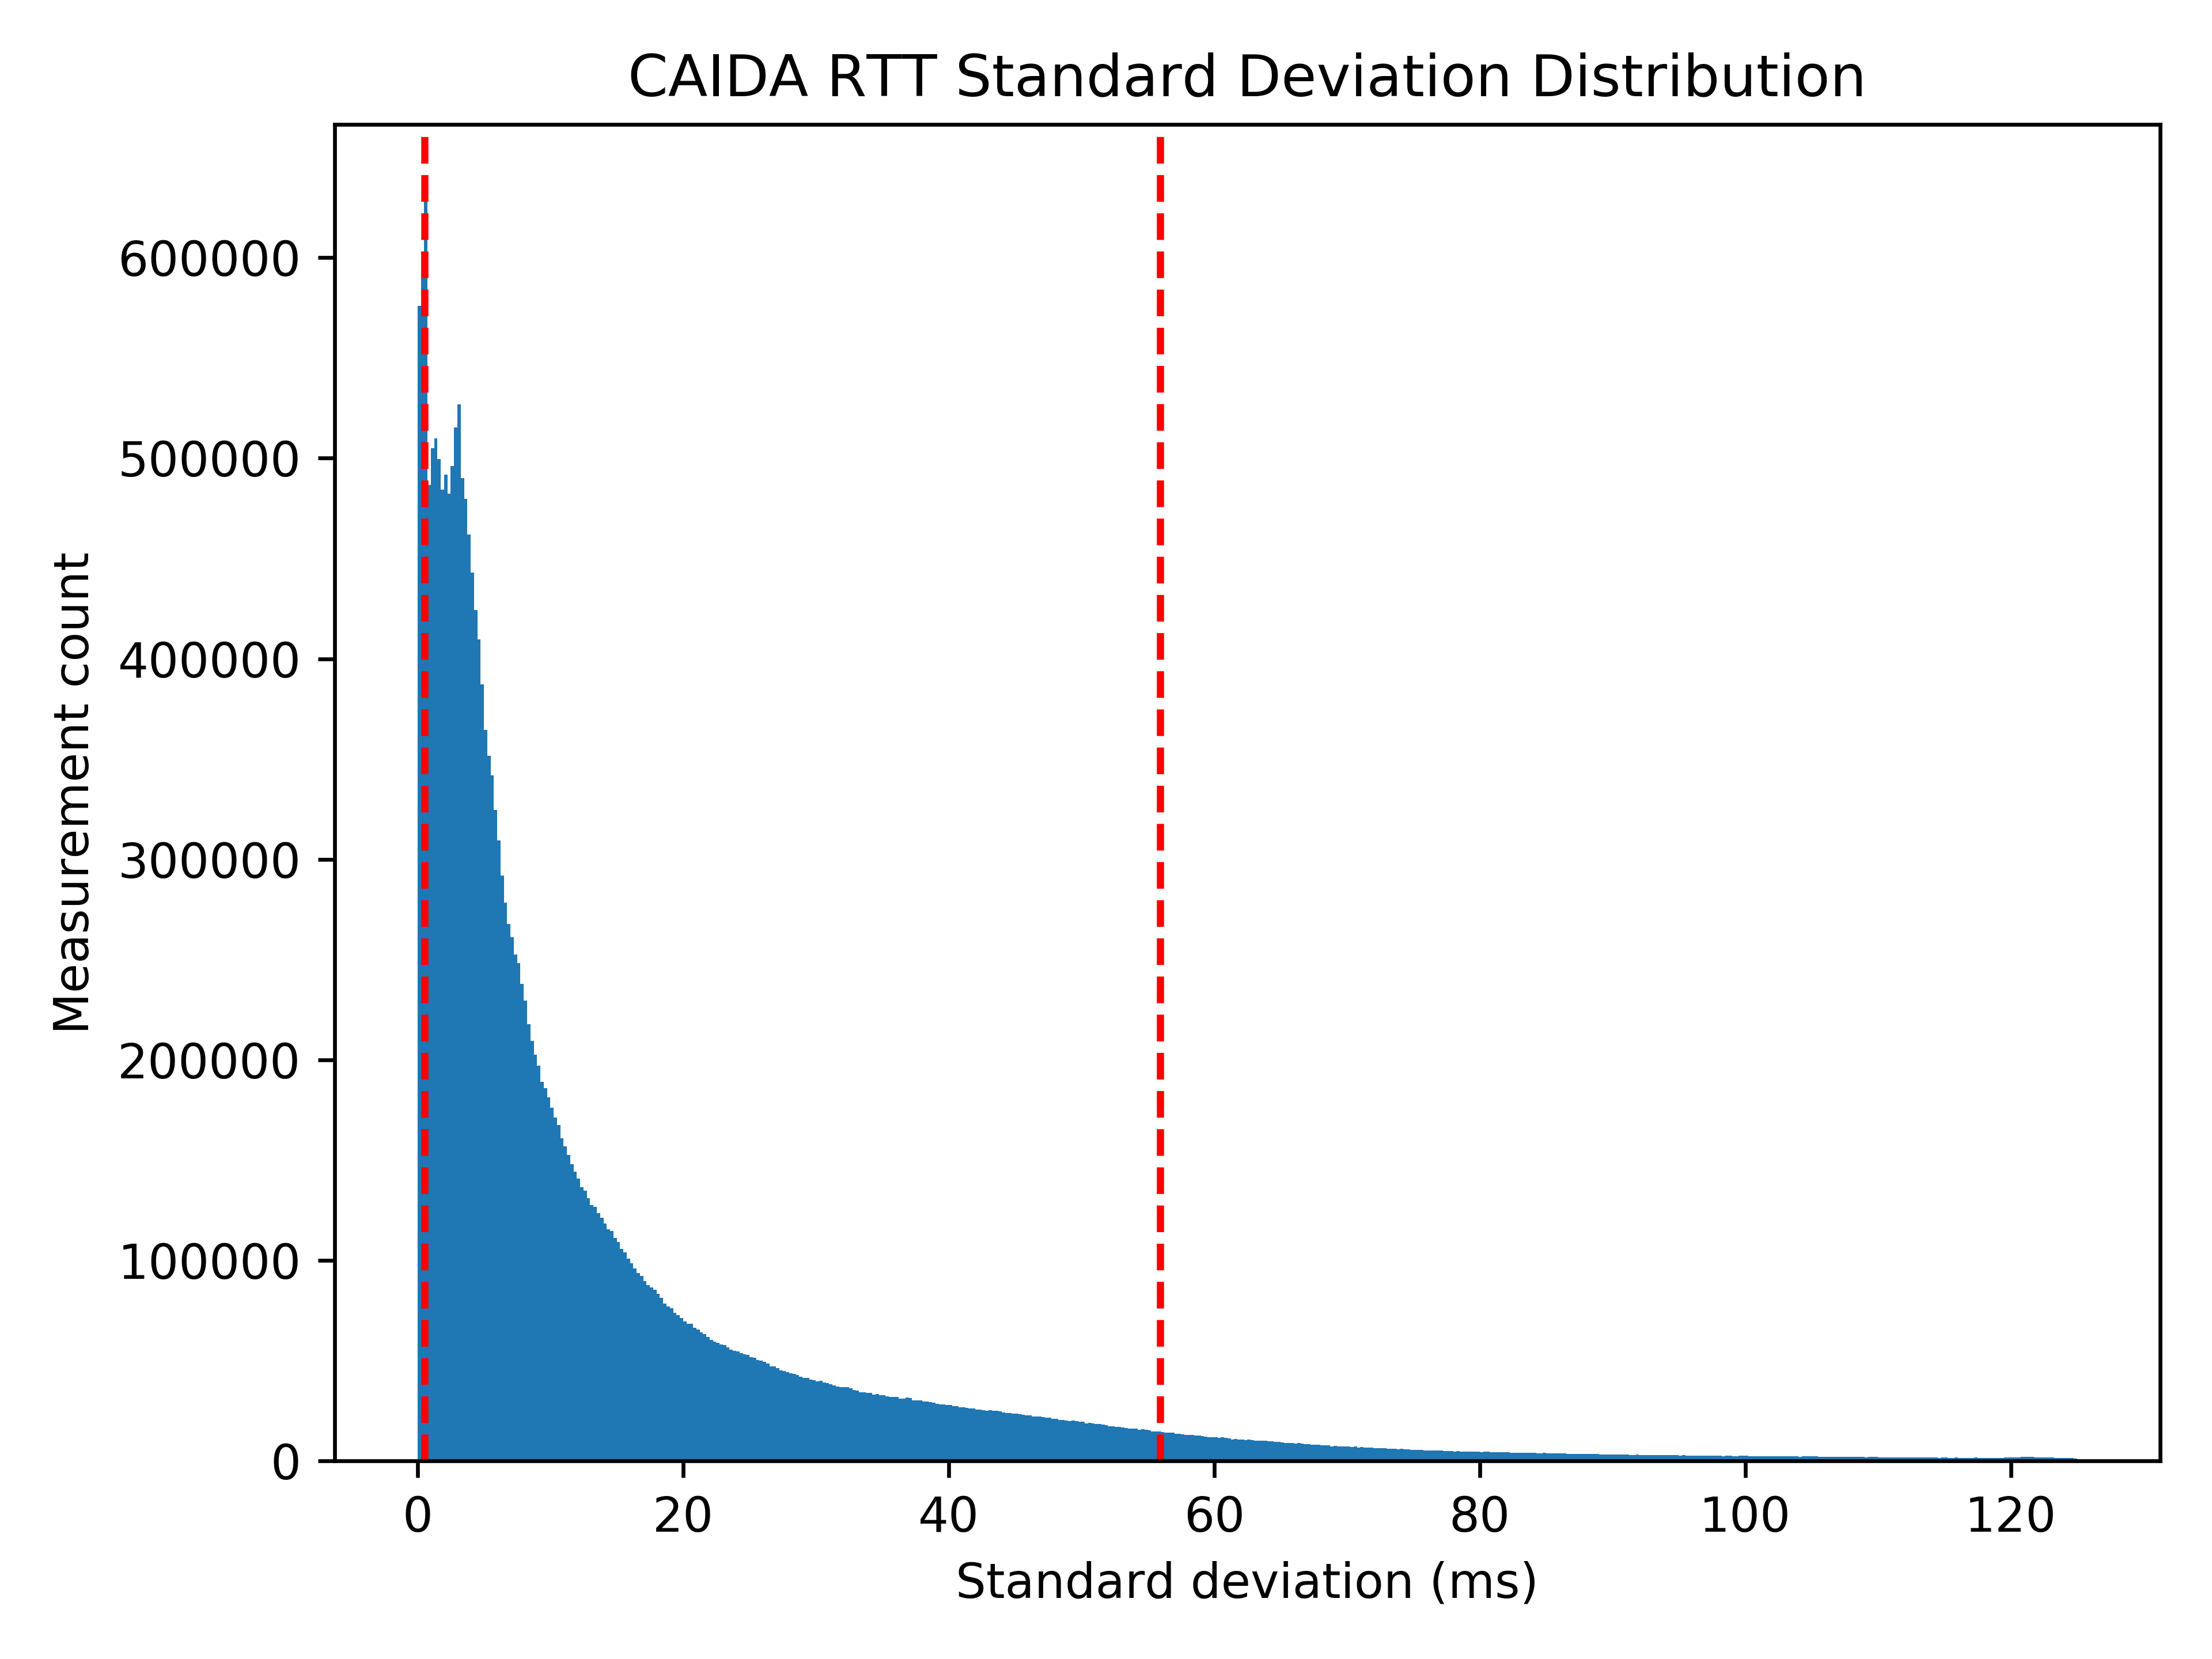
\includegraphics[width=\textwidth]{CAIDA_rtt_stdev_dist.png}
    \caption{Distribution of CAIDA RTT standard deviations with 5th and 95th percentiles}
    \label{fig:rtt_stdev_dist}
\end{figure}

Since \caida reports many trials per source-destination pair, a measure of the standard deviations of those measurements is useful to gauge jitter along connections. Figure \ref{fig:rtt_stdev_dist} shows the distribution of standard deviations, which shows a beautifully sloped curve that peaks on the left -- lower standard deviation means lower spread of data, so we can reasonably infer the data is of high quality.

\begin{figure}[H]
    \centering
    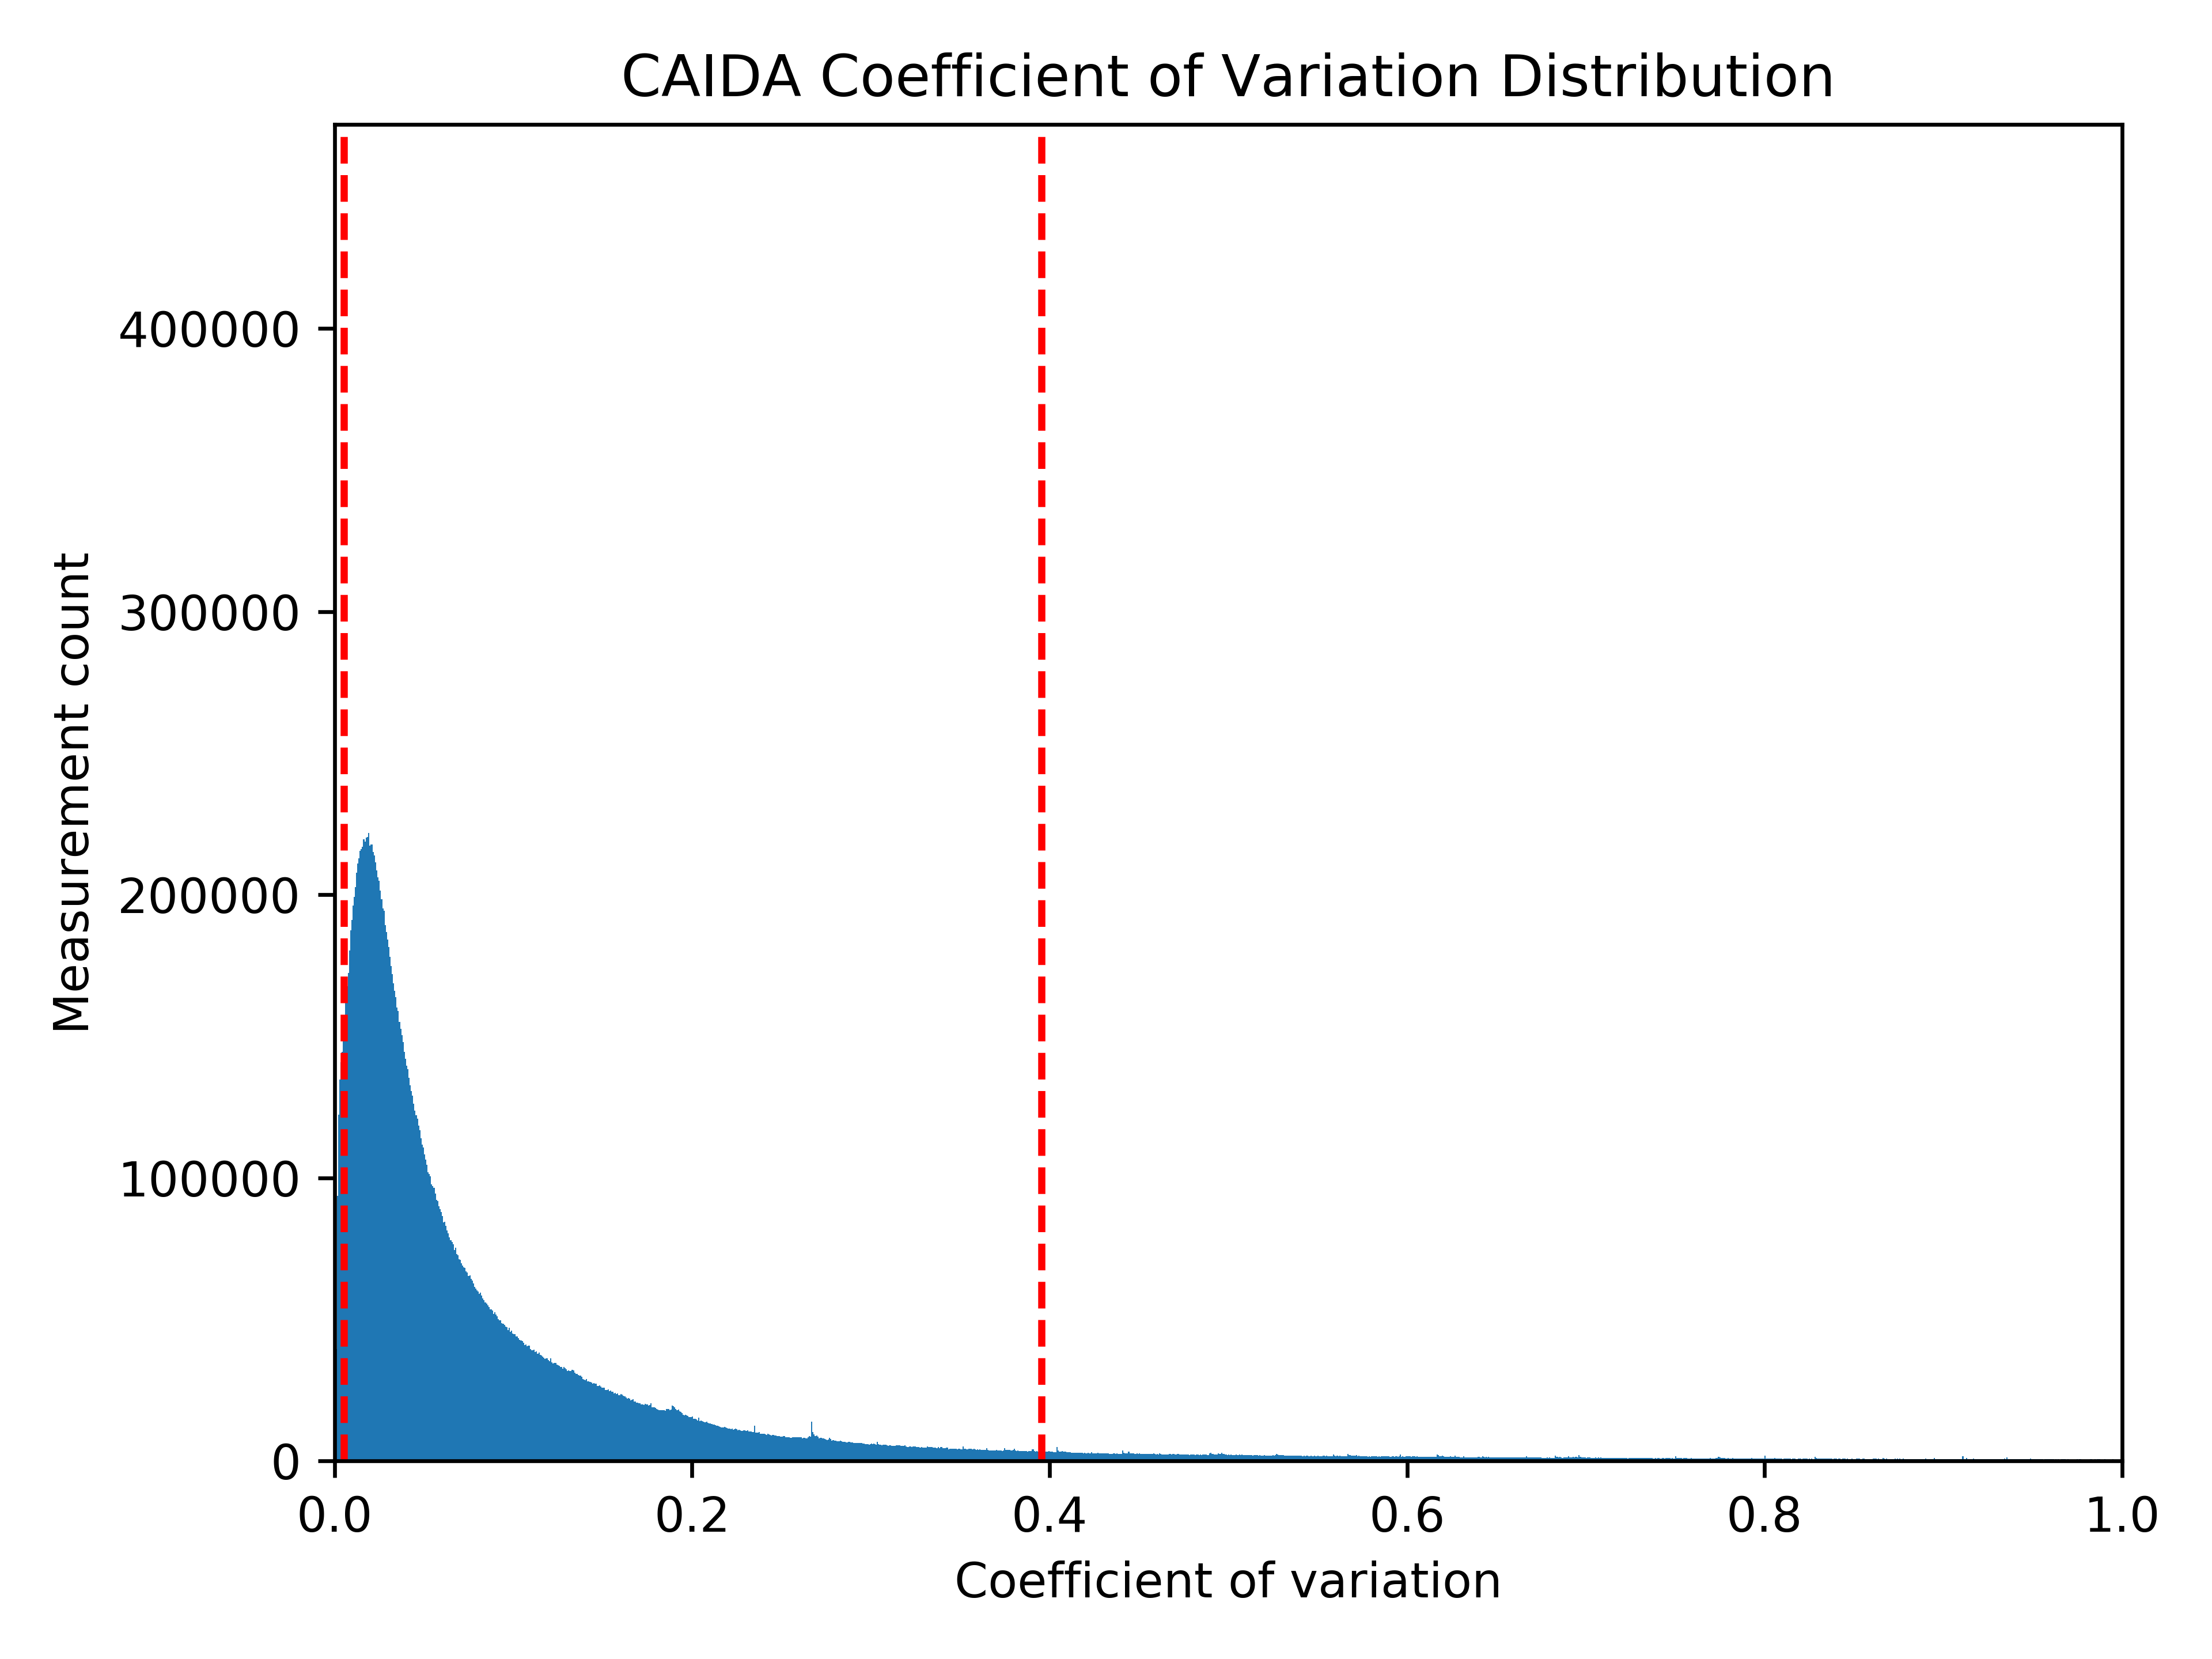
\includegraphics[width=\textwidth]{CAIDA_cv_dist.png}
    \caption{Distribution of CAIDA RTT coefficients of variance with 5th and 95th percentiles} 
    \label{fig:rtt_cv_dst}
\end{figure}

To compound on that, figure \ref{fig:rtt_cv_dst} shows a distribution the \glspl{cv} for the data set, dimensionless values that can be interpreted the same regardless of the underlying data. These are calculated by dividing the standard deviation by the mean, so lower is better. Broadly speaking the majority of the data is of excellent quality, but this information is definitely useful on setting appropriate limits for filtering.

\subsubsection{Raw RTT}
Combined, these three data sets give us access to huge amounts of data on the \rtts between nodes everywhere in the world -- hundreds of millions of machines -- both for end-to-end connections and connections to intermediaries. Since there are many traceroutes for each source-destination pair, we can control for jitter by averaging measurements together and reporting on other common statistics values (range, standard deviation, etc).

Each \ip in the data set can be geo-located to provide us with reasonably accurate locations for every \ip that appears in the dataset. These locations plus the \rtts can be used to build a heat map that shows what average \rtt looks like from any given location in the US. Filtering can be done to further refine this, e.g. average \rtt to only US servers, only international servers, and so on.

\subsubsection{RTT per distance}
\rtts naturally vary with distance, both because the number of nodes in the path tends to increase with path length (increasing routing delays) and because time to get data from point A to point B is governed by the speed of light. The amount an \rtt varies with distance, though, depends on the quality of the infrastructure between connection endpoints, so \rtt divided by distance (in units of ms/km) is a good metric for understanding internet connectivity.

To that that end we've conducted some early data analysis using a subset of the \caida prefix probing dataset, and have generated the following heatmap:

\begin{figure}[H]
    \centering
    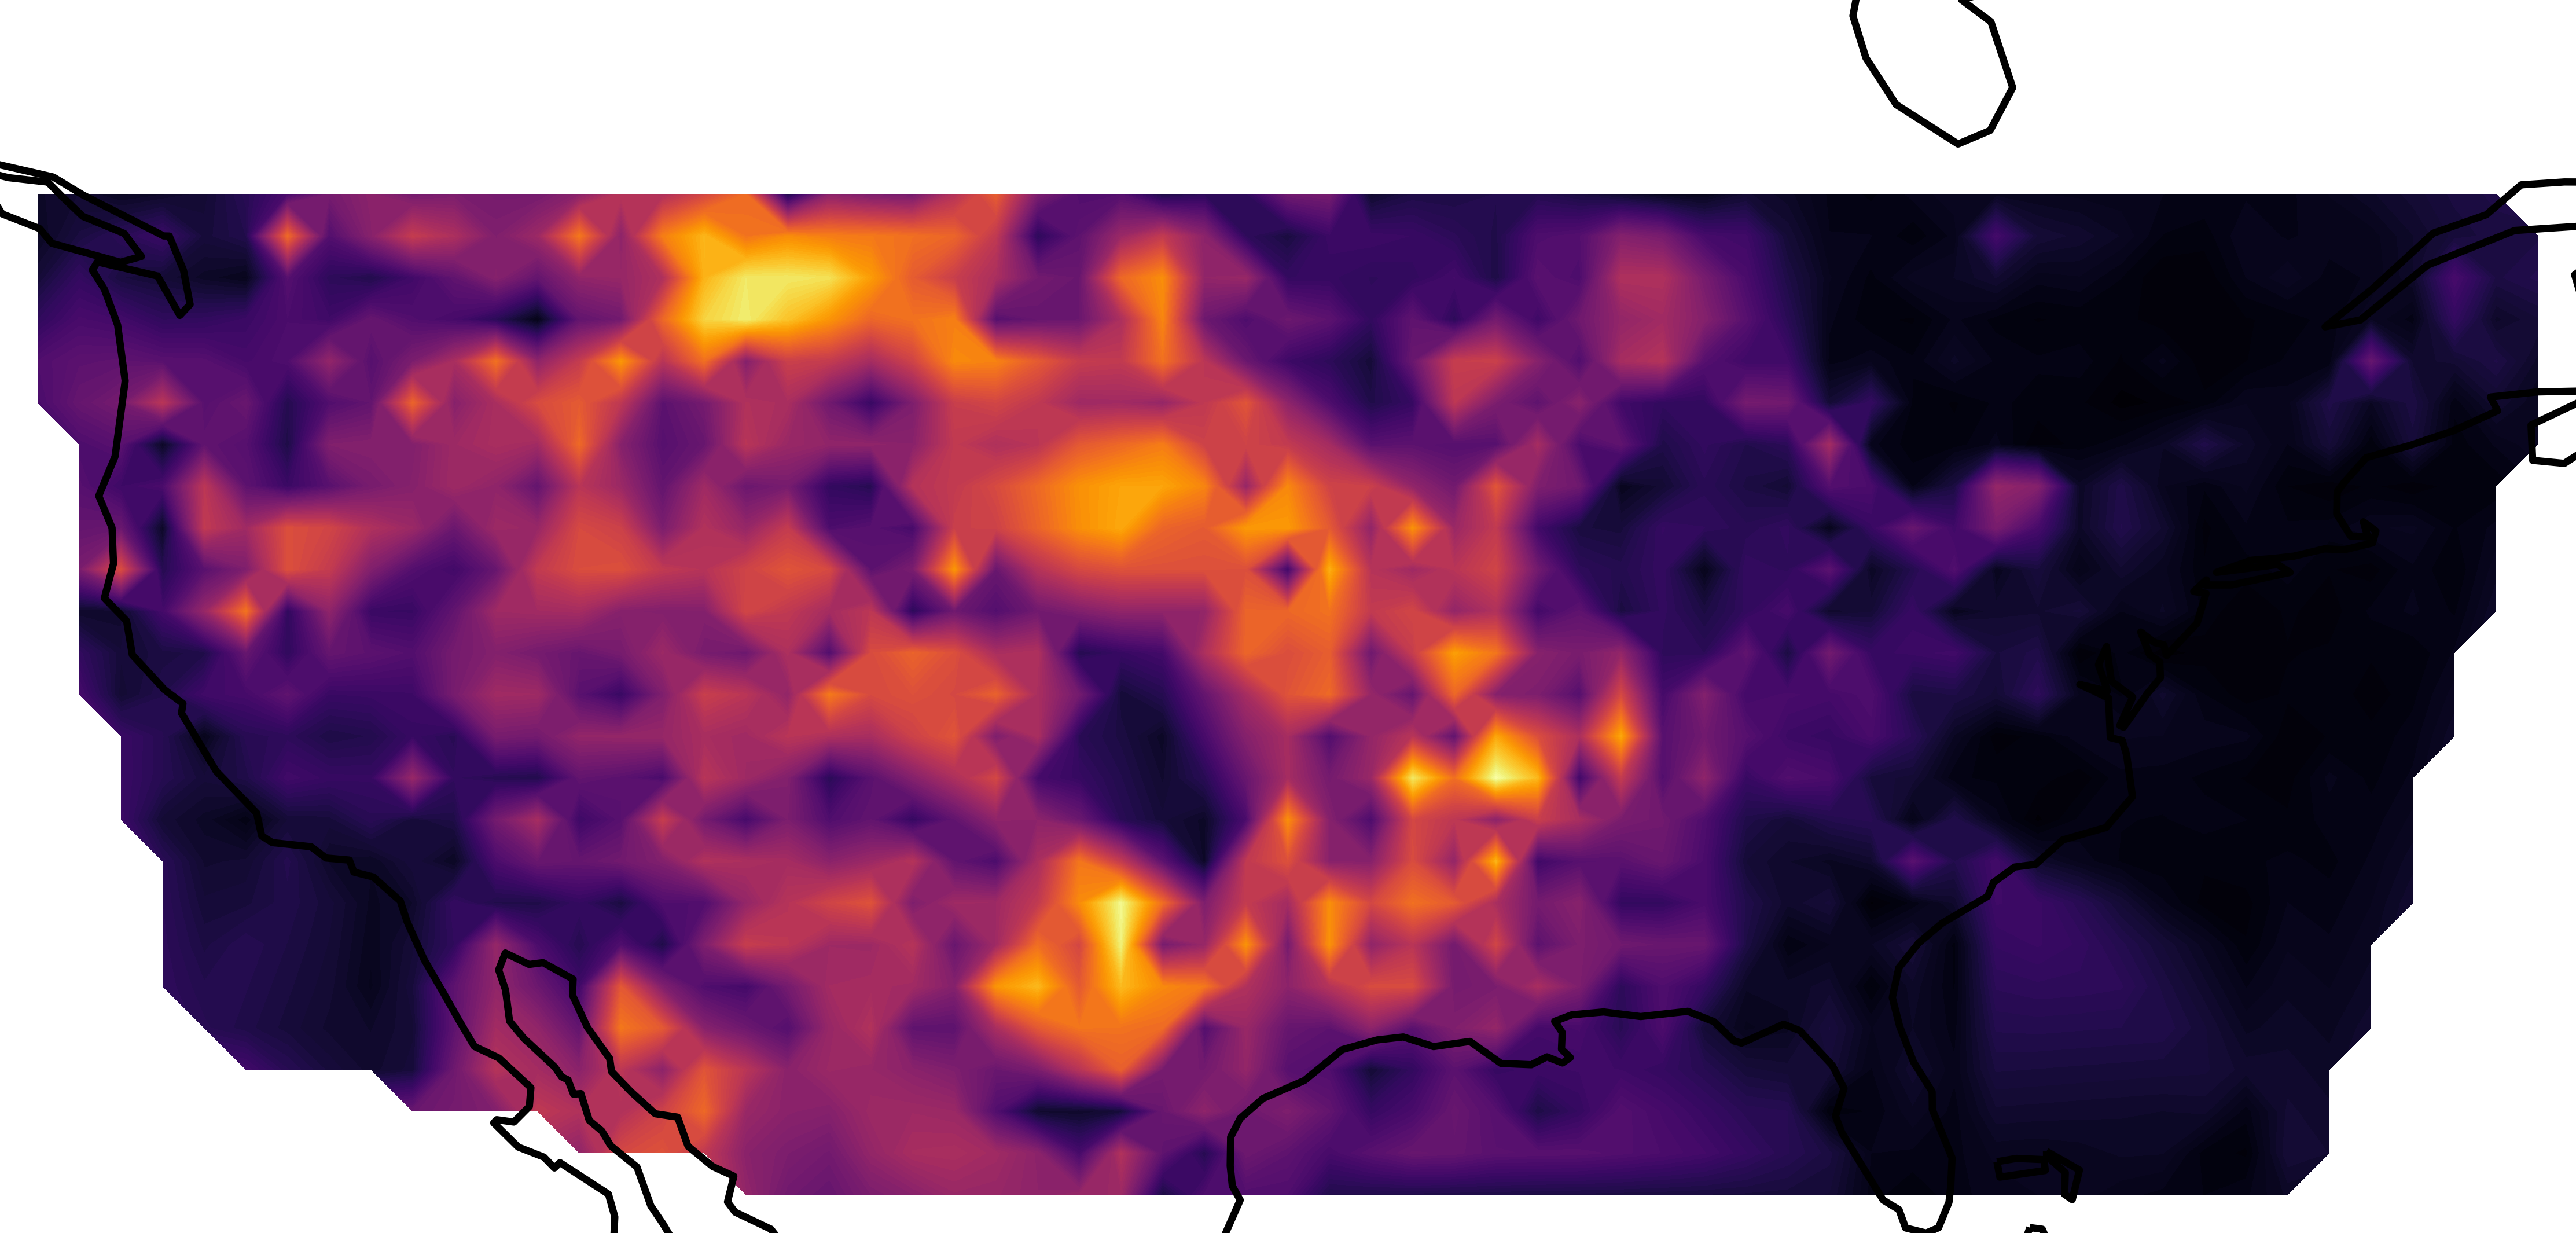
\includegraphics[width=\textwidth]{CAIDA_connect_heatmap.png}
    \caption{Heatmap of ms/km values}
    \label{fig:caida_connectivity_heatmap}
\end{figure}

Figure \ref{fig:caida_connectivity_heatmap} shows a heatmap of connectivity across the US where brighter areas correspond to lower internet connectivity. This roughly corresponds to data available from \isps, which indicate that the Northwest, for instance, generally has much poorer internet access. This map was generated using python matplotlib and some data analysis techniques to reduce the sheer quantity of data from hundreds of millions of data points to only a few thousand (see \S{}\ref{sec:optimization}).

\begin{figure}[H]
    \centering
    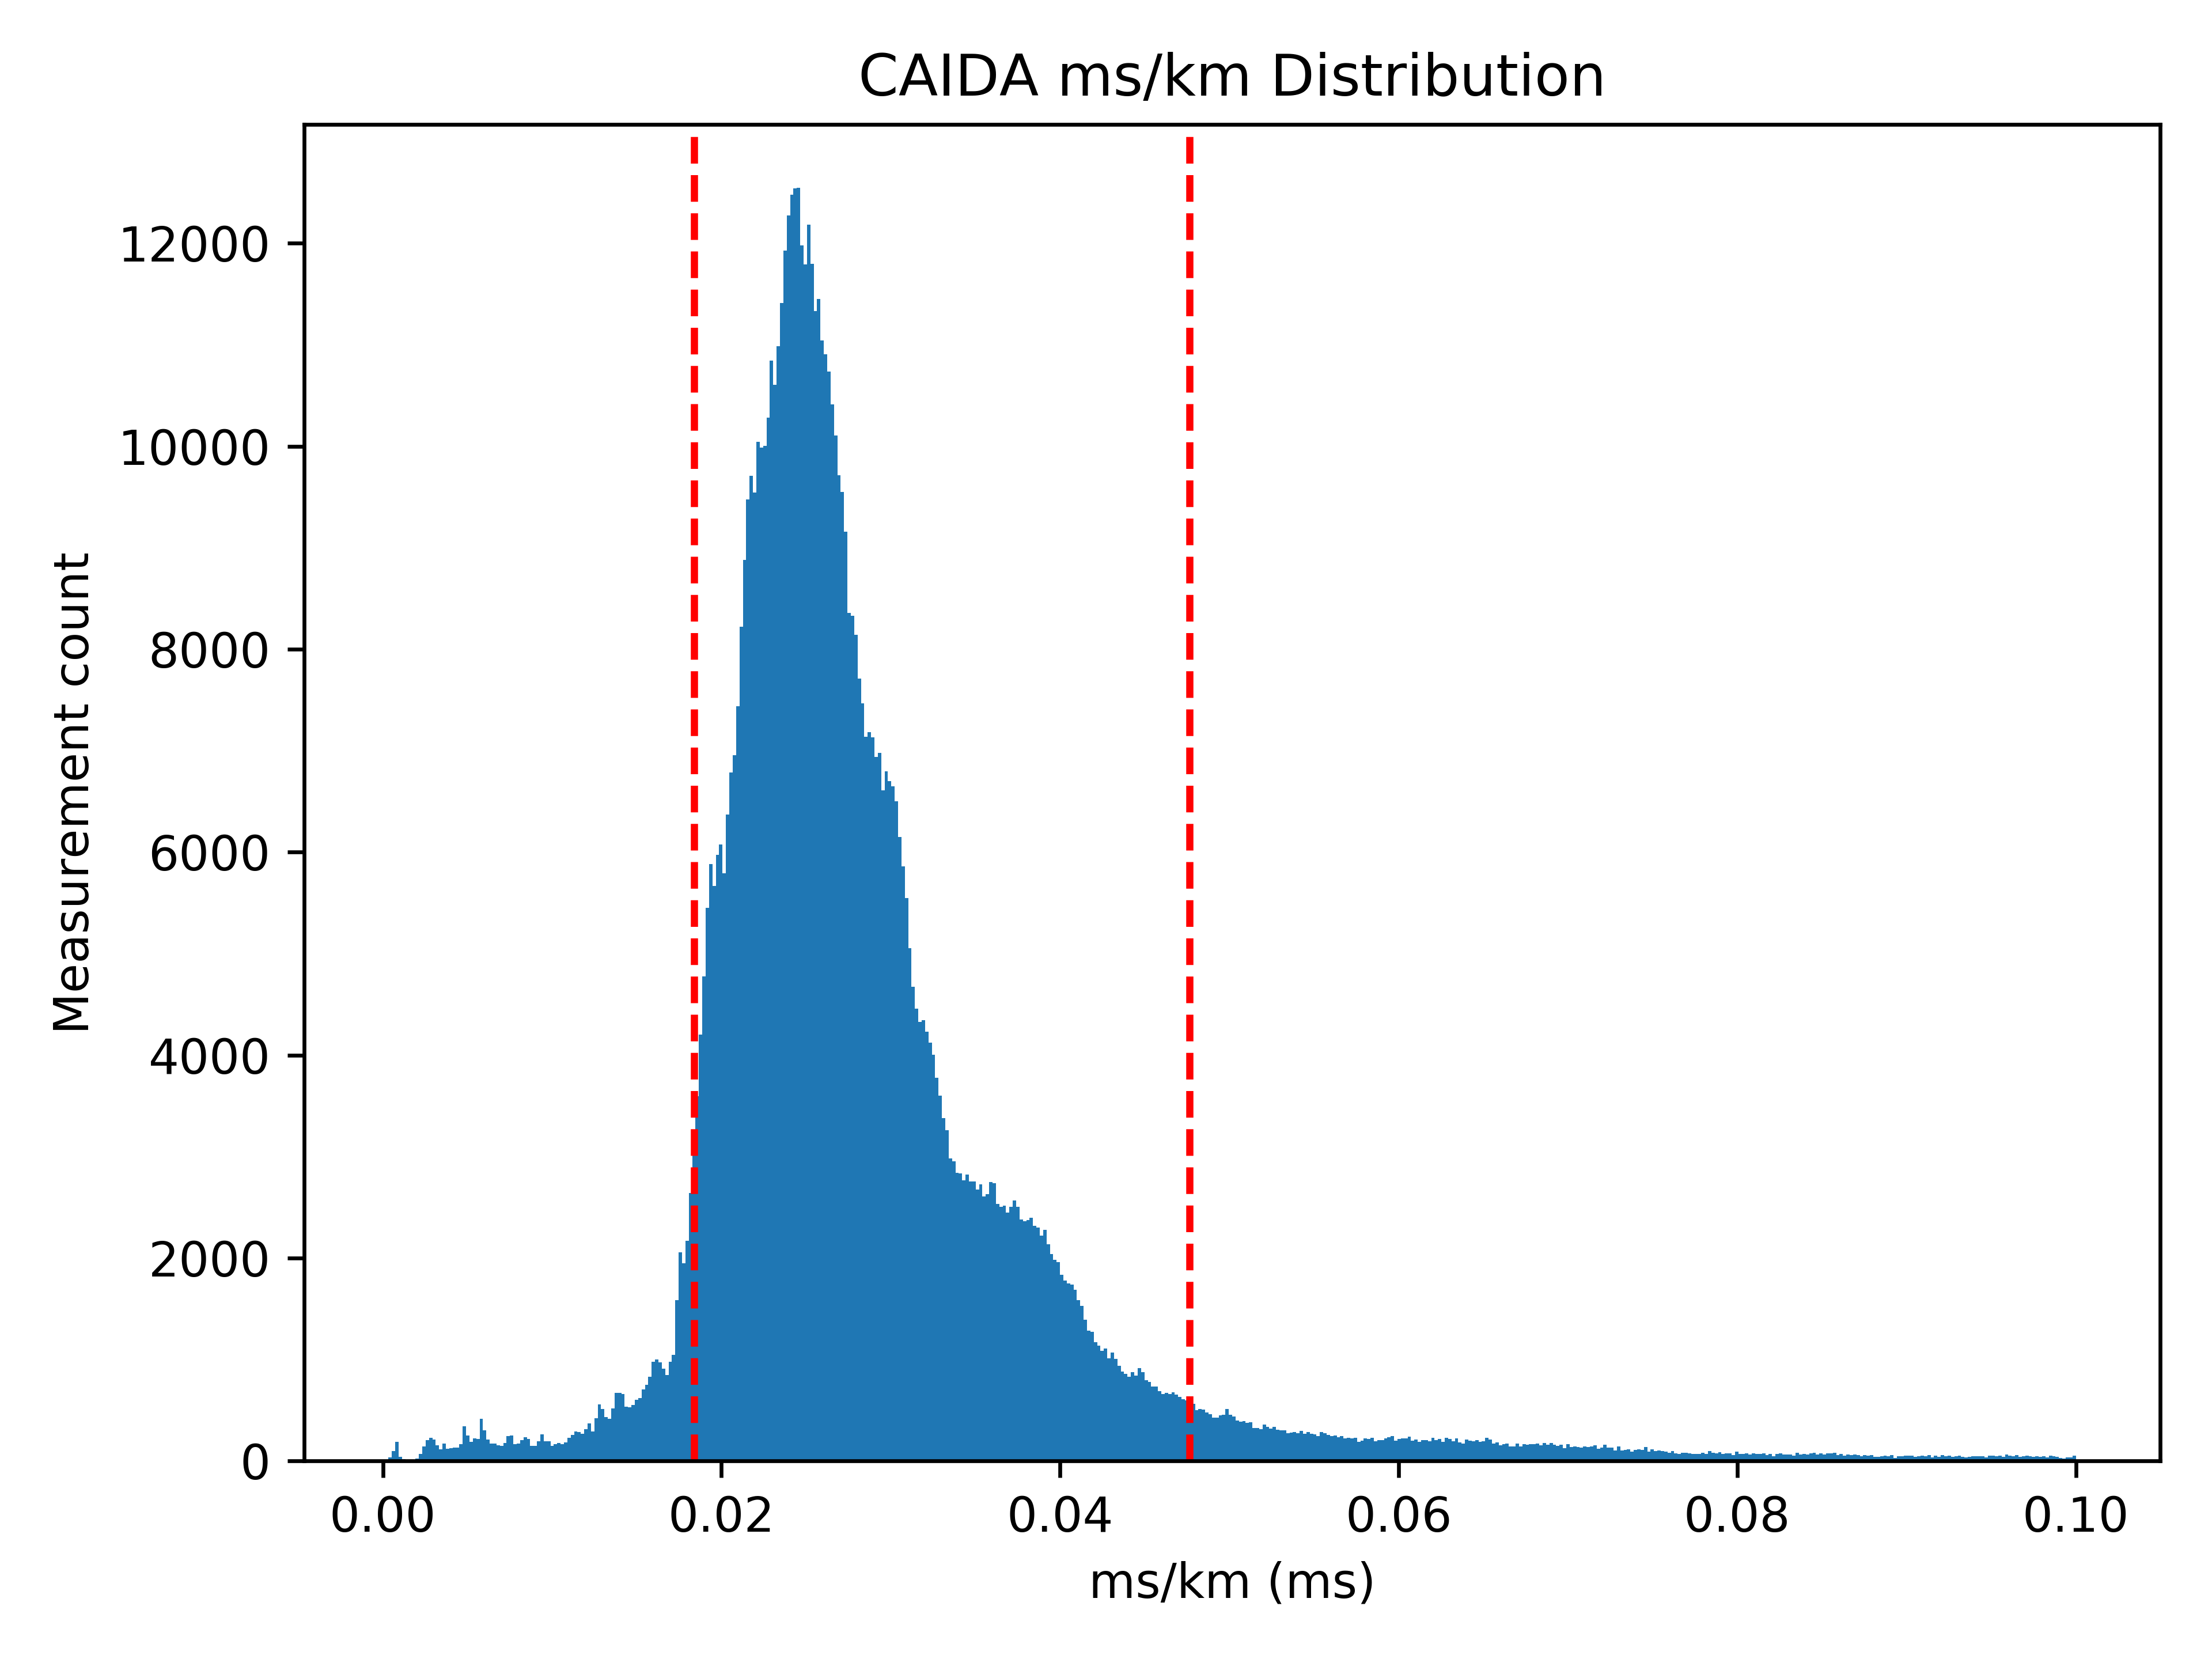
\includegraphics[width=\textwidth]{CAIDA_connect_dist.png}
    \caption{Distribution of CAIDA ms/km values with 5th and 95th percentiles}
    \label{fig:caida_connectivity_dist}
\end{figure}

Figure \ref{fig:caida_connectivity_dist} shows is based on the data as figure \ref{fig:caida_connectivity_heatmap}, but shows a distribution instead. This is another fairly narrow peak, but with enough interesting variation and shoulders to hint at underlying patterns and data worth analyzing.

\subsubsection{Backbone analysis}

The benefit to collecting traceroutes instead of direct pings is that we obtain an ordered list of all nodes between endpoints. This forms a simple linear directed graph for each traceroute; by finding common source/destination pairs between traceroutes we can add to the graph. Series of pairs that are very commonly traveled can be automatically inferred to be backbone connections that great portions of traffic travels through. By identifying these nodes we can extract information on how long it takes each node in the graph to reach the nearest identified backbone node. This should provide useful insight on internet connectivity, since connection speed to the nearest major internet exchange likely has a much greater influence on connectivity than does the ability of a given node to connect to any other node.

\subsubsection{Direct RTT, route RTT, \& calculated hop RTT}

For each traceroute there are three modes of analysis: direct ping, all pings, and hop ping calcuation. A direct ping just means discarding all intermediary hops and only considering \rtt to the target node, hence being equivalent to a direct ping. Considering all pings in a traceroute means recording \rtt to each individual node. That is, if you have $A\rightarrow B\rightarrow C\rightarrow D$, you record data for $A\leftrightarrow B, A\leftrightarrow C$, and $A\leftrightarrow D$. These in turn correspond to actual ping-equivalents received from the remote node.

Calculated hops are more complicated. For each hop along the route an \rtt value is recorded, e.g. $B=5, C=12, D=25$. By subtracting each node's \rtt from the \rtt of the node \textit{ahead} of it, we can estimate the \rtt from the first node to the second. So in this case, we would calculate $B\leftrightarrow C=7$ and $C\leftrightarrow D=13$. These values are approximate since we don't have a direct measurement, but useful all the same in calculating the quality of individual links. 

By combining the three methods, for a traceroute with $n$ hops we obtain $2n-2$ datapoints. 

\label{sec:optimization}\subsubsection{Optimization Techniques \& Database Design}

To put it mildly, there is a \textit{massive} amount of data to analyze. We estimated about 185 billion datapoints from \caida alone using one method of analysis; even if it's off by an order of magnitude or two, we're still dealing with datapoints in the billions. This amount of raw data is clearly impossible to plot all in one graph, and even if we did, the data would be minimally useful. To that end we've devised a few basic methods for reducing the size of the dataset into something more manageable, without compromising the meaning behind the data. Some of these methods are common statistics and data science techniques, some are not.

\paragraph{Grouping source-destination pairs}

We interpret multiple instances of source to destination pairs as the equivalent of multiple "trials" of an experiment. These values are grouped together and averaged to create a final value. We also calculate the standard deviation and range of the values that formed the average.

\paragraph{Filtering by coefficient of variation}

The coefficient of variation is an ideal quantity for filtering as it doesn't matter what the underlying data set is. We can reduce the data by filtering to source-destination pairs with CVs below 20, for example.

\paragraph{Storing location and IPs separately}

Performing a geo-IP lookup is costly, so caching is preferable. Storing source+destination latitude and longitude alongside each source-destination pair is also costly, with a minimum of 16 extra bytes per row, and when you're dealing with billions of rows, every byte counts. To solve this, locations are cached in a separate table that is joined with the filtered and grouped \glspl{ip} instead of with locations for each raw data point.

\paragraph{Quadtree grouping}

The above methods can reduce a \textapprox{}200,000,000 row table to only \textapprox{}800,000 rows, a massive improvement but still too much to chart at once. To solve this we devised a quadtree-based algorithm for grouping nearby points together and averaging them. This is based on the premise that close-together measurement points \textit{should} have roughly similar values. We can't just divide the map into an equally-spaced grid, though, as that would lose a lot of nuance in the data.

The quadtree algorithm works by first assembling a list of all datapoints, finding medians along the horizontal and vertical axes, and splitting into four groups based on those values. The same process is repeated recursively for each child group, with the necessity of a further split determined by exceeding some set level of items, and up to a maximum tree depth that corresponds to the granularity of the resulting map. When put into action and graphed directly, the resulting map looks something like this:

\begin{figure}[H]
    \centering
    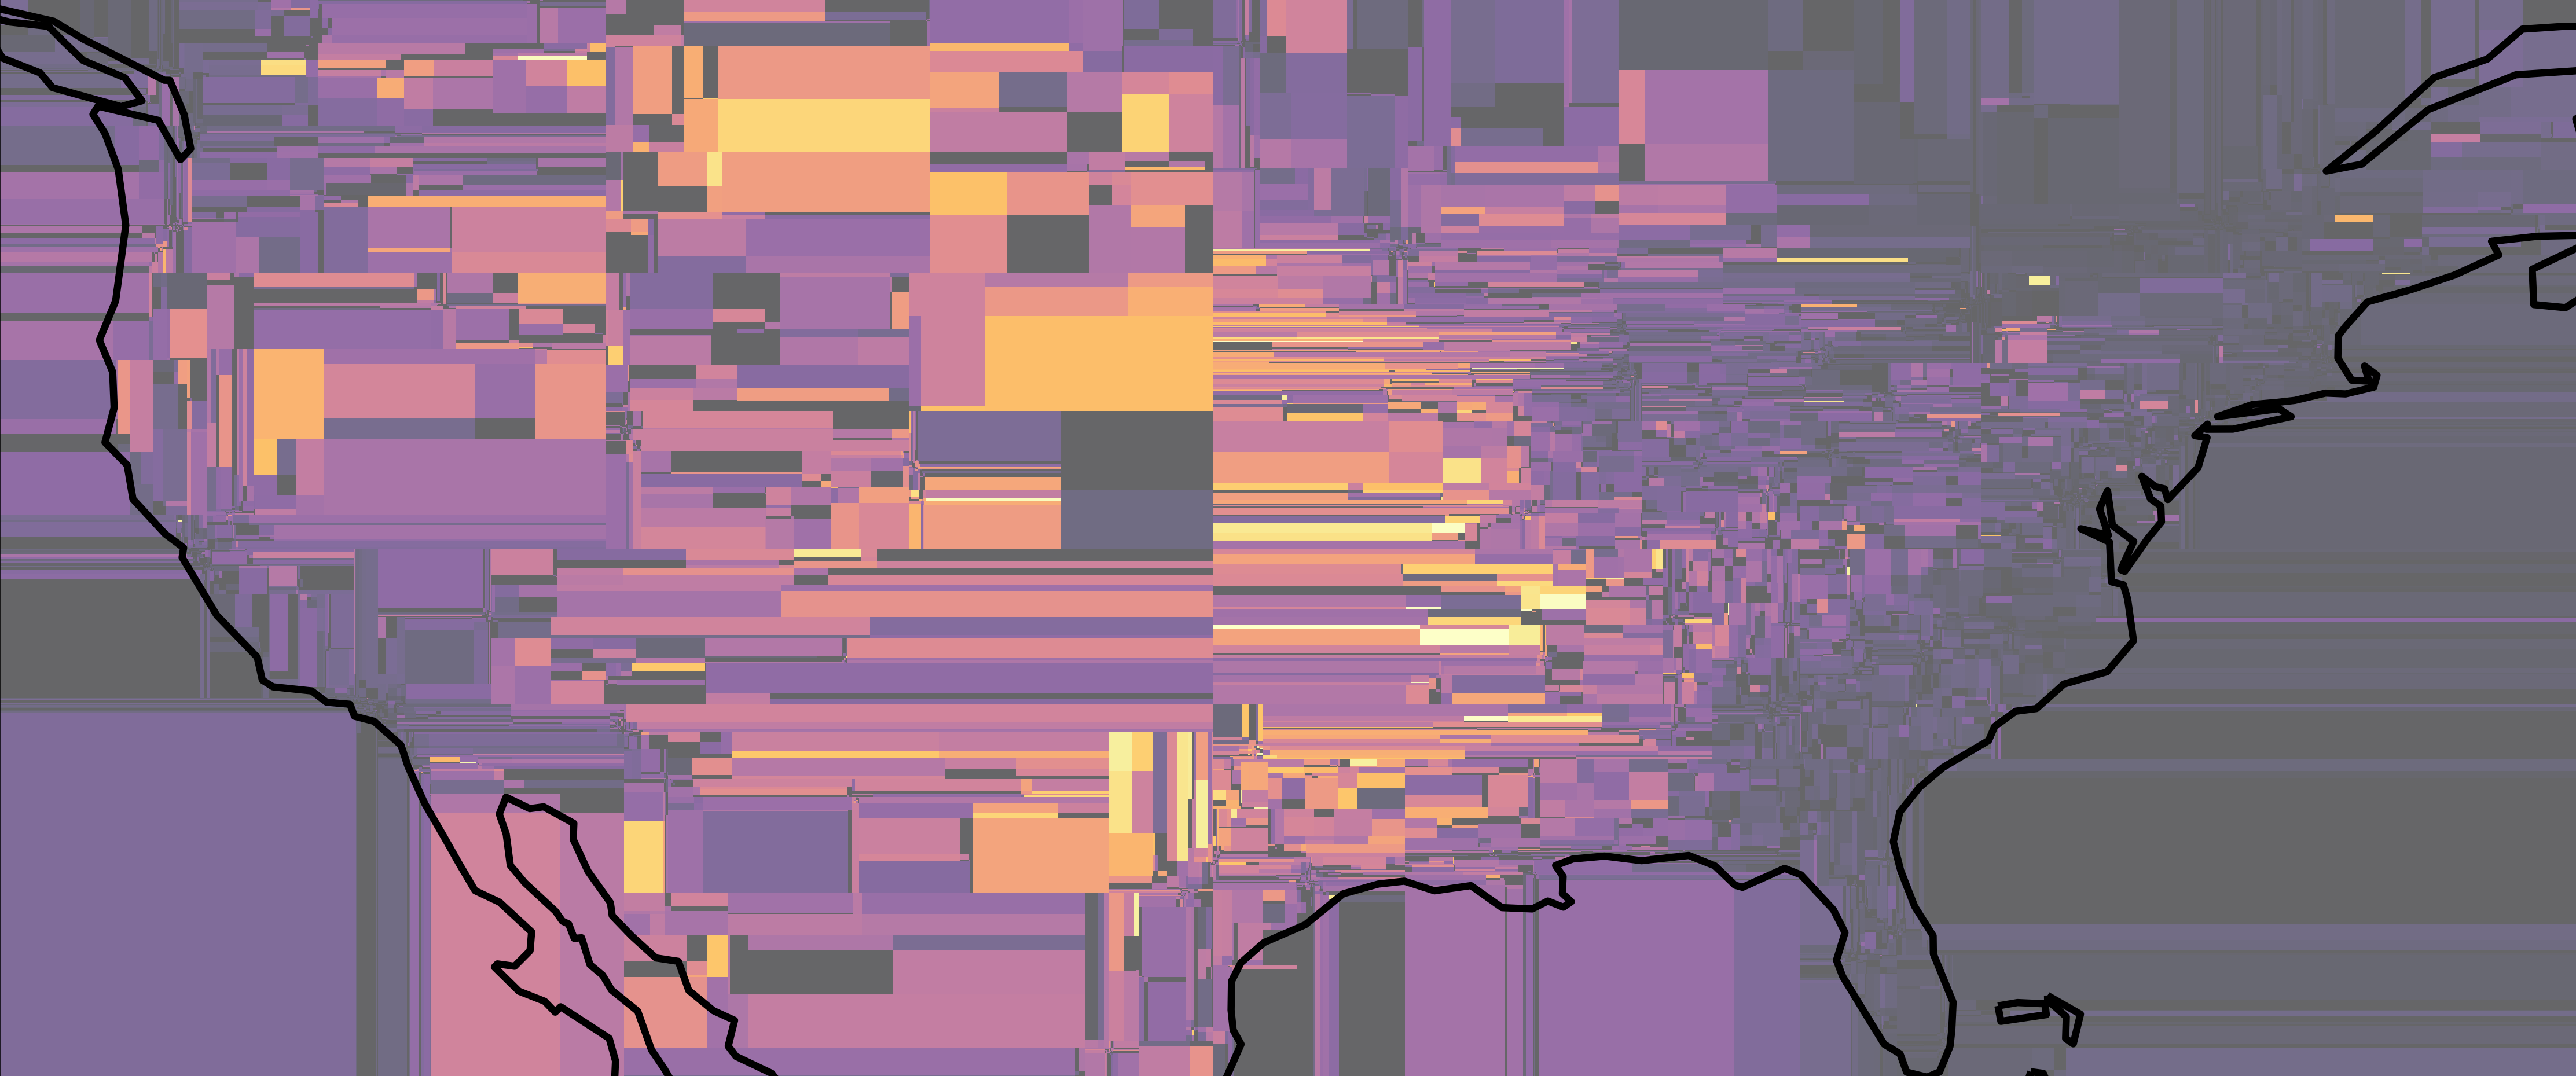
\includegraphics[width=\textwidth]{images/CAIDA_connect_quadplot.png}
    \caption{Ms/km heatmap, quadtree format. Brighter areas indicate higher values.}
    \label{fig:caida_quadplot}
\end{figure}

The smaller the box, the more measurements are in that geographic area. The center of the box is interpreted as a data point and graphed accordingly. Using this technique, the total amount of data points can be reduced from hundreds of thousands to under 1,000, with an average efficiency of about 90\%. This technique was used to generate the heatmap shown in figure \ref{fig:caida_connectivity_heatmap}.

    \subsection{ISP mapping}[David V.]
Using the \fcc's comprehensive Fixed Broadband Deployment database \cite{FederalCommunicationsCommission} we can see what the maximum rated connection speed that is offered in each zip code, as well as the number of \isp that serve a given area. Another useful data collection method  for this could be asking users on a distributed website what there rated connection is, and that number can be compared to the "Rated" maximum speed. 

\subsubsection{Rated connection speed for given location speed}
By mapping the rated connection speed for the given location you can get an idea of the "advertised" connection speeds across the country. This data would be useful for users, especially when compared to the measured speeds from the favicon pings or the \caida data. Comparing these measured data points to the advertised data points could also give people an idea if they are able to get what they are paid for.  

    \subsection{Route-trip}[Evan G.]
Using an application on either a mobile device (e.g. smart phone or laptop equipped with mobile broadband and \acrshort{gps}), we could drive across any given area (up to the entire continental United States) and run traceroutes or pings to \ip addresses/domain names for top sites, and record the \rtt along with an exact location. The information collected could be used to measure both cellular infrastructure and 4G connectivity as well as local internet connectivity.

    
    
    %%%%%%%%%%%%%%%%%%
    %%% END MATTER %%%
    %%%%%%%%%%%%%%%%%%
    
    % It's simpler to disable automatic sectioning for the glossaries and references than it is to fix a bug
    % in table-of-authorship handling. I'm so, so sorry.
    \singlespacing
    \let\endsection\section
    \renewcommand{\section}[2]{}%
    
    % List of acronyms
    % \footnotesize
    \newpage
    \endsection{Acronyms}
    \setglossarystyle{mcolindex} % See https://www.dickimaw-books.com/gallery/glossaries-styles/ for styles
    \printglossary[type=\acronymtype]
    
    \endsection{Glossary of terms}
    \setglossarystyle{index}
    \printglossary
    
    % Bibliography, automagically managed in IEEE style.
    \newpage
    \nocite{*}
    \endsection{References}
    \printbibliography
\end{document}